% METODOLOGIA------------------------------------------------------------------
\chapter{PROCEDIMENTOS METODOLÓGICOS}
\label{chap:metodologia}

Este capítulo tem como finalidade descrever a metodologia e os procedimentos adotados na confecção deste projeto, bem como também realizar uma consolidação de todos os métodos aqui utilizados e apresentar o funcionamento do sistema como um todo. Para tal, os procedimentos metodológicos foram divididos da seguinte forma: Fonte inversora (Seção 3.1), DSPIC33E  (Seção 3.?)

\section{FONTE INVERSORA}
\label{sec:fonteInversora}

Para realizar a alimentação do magnetron, foi utlizada uma fonte inversora, a qual consiste em um inversor ressonanete classe E. Segundo \cite{Hidenori1991}, uma fonte inversora tem as seguintes vantagens em relação à uma fonte ferrorressonante tradicional:
\begin{itemize}
    \item Potência de saída controlável;
    \item Maior eficiência energética;
    \item Circuito menor e mais leve;
    \item Pode operar em maior frequência.
\end{itemize} 

\begin{figure}[!htb]
    \centering
    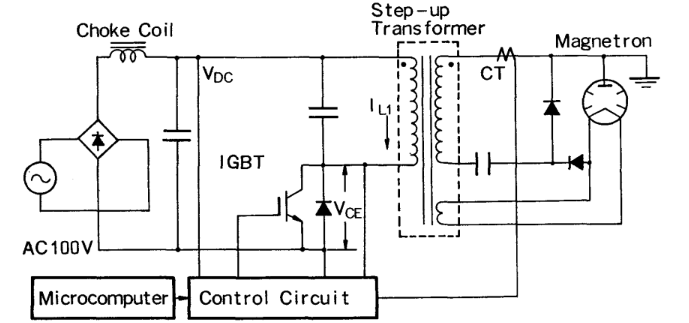
\includegraphics[width=0.9\textwidth]{./dados/figuras/font_inverter}
    \caption{Fonte inversora para alimentação do magnetron}
    \fonte{\citeonline{Hidenori1991}}
    \label{fig:figura-inverter}
\end{figure}

\subsection{Simulações}
\label{sec:simulations}

Para verificar se a fonte inversora é viável para o projeto, foram feitas simulações do circuito no software \textit{PSIM}. Na alimentação o magnetron, são necessários cerca de 4 kV. Assim, primeiramente foi desenvolvido um circuito para simular a alimentação de uma carga de cerca de 100 M$\Omega$, com uma tensão de entrada de 127 V. A figura a seguir mostra o circuito desenvolvido:

\begin{figure}[!htb]
    \centering
    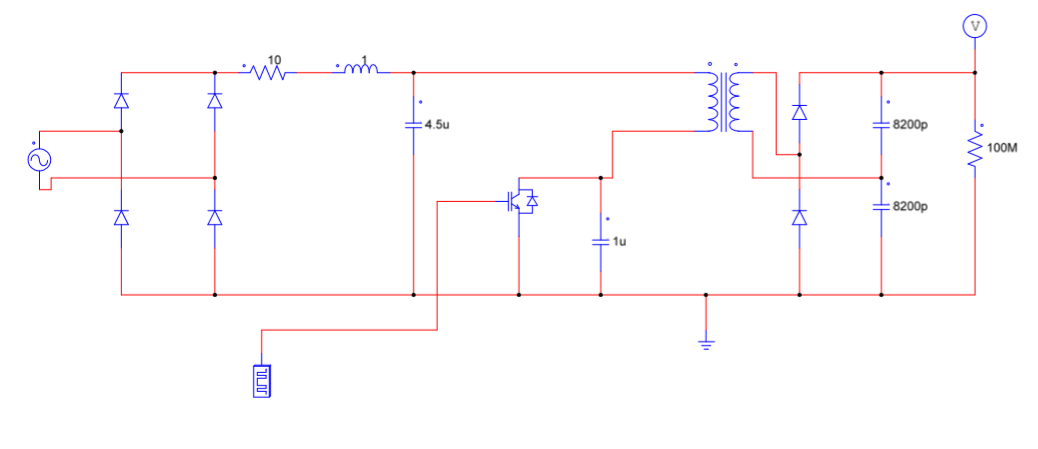
\includegraphics[width=0.9\textwidth]{./dados/figuras/psim1}
    \caption{Circuito da fonte inversora simulada}
    \fonte{Autoria própria (2019)}
    \label{fig:circ_sim_1}
\end{figure}

Para averiguar se uma fonte inversora consegue alimentar uma carga de alta potência à uma tensão de alguns kV, o inversor foi chaveado em um ciclo de trabalho de 50\%. A figura abaixo mostra a froma de onda da tensão na carga resistiva:

\begin{figure}[!htb]
    \centering
    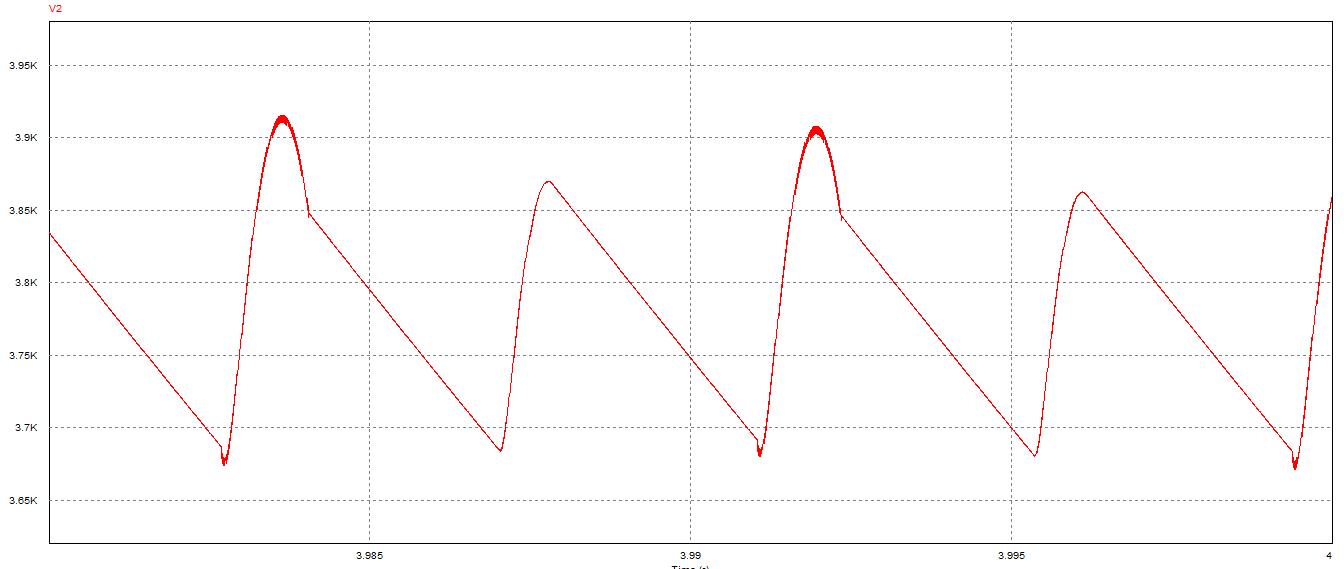
\includegraphics[width=0.9\textwidth]{./dados/figuras/psim2}
    \caption{Forma da onda simulada da tensão na carga}
    \fonte{Autoria própria (2019)}
    \label{fig:figura-graf_sim_1}
\end{figure}

Na figura \ref{fig:figura-graf_sim_1}, pode-se ver que o pico de tensão da carga chega a quase 4 kV o que já é suficiente para o objetivo em questão. Logo, conclui-se que a fonte inversora é viável para a alimentação do circuito de um magnetron.

\section{DSPIC33E}
\label{sec:dsPIC}

O DSPIC33E é um microntrolador da família PIC, desenvolvido pela Microchip Technology Inc., que possui suporta a fucnionalidade de processador digital de sinais (DSP). Este componente foi escolhido para fazer o controle do chaveamento da fonte inversora pois o mesmo consegue operar em uma ampla faixa de temperatura e possui diversas funcionalidades interessantes para o controle de sinais analógicos de alta frequência. Algumas das funcionalidades, cruciais para o projeto, incluem:
\begin{itemize}
    \item
    \item Três comparadores/amplificadores operacionais com conexão direta ao ADC da plataforma;
    \item Interrupções de \texit{Change Notification} em todos os pinos de I/O;
    \item Funções de PWM de alta velocidade;
    \item Circuito menor e mais leve;
    \item Pode operar em maior frequência.
\end{itemize} 

\begin{figure}[!htb]
    \centering
    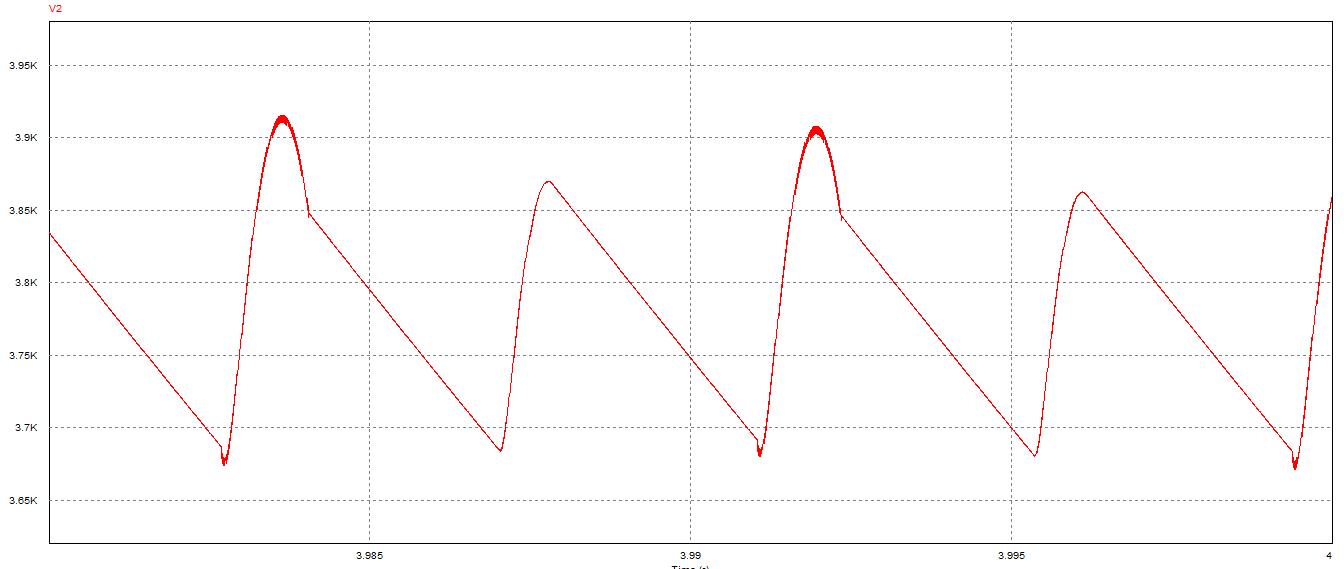
\includegraphics[width=0.9\textwidth]{./dados/figuras/psim2}
    \caption{Forma da onda simulada da tensão na carga}
    \fonte{Autoria própria (2019)}
    \label{fig:figura-graf_sim_1}
\end{figure}

No tocante ao microprocessador da plataforma, o mesmo...



